\begin{figure}[!htb]
    \centering
    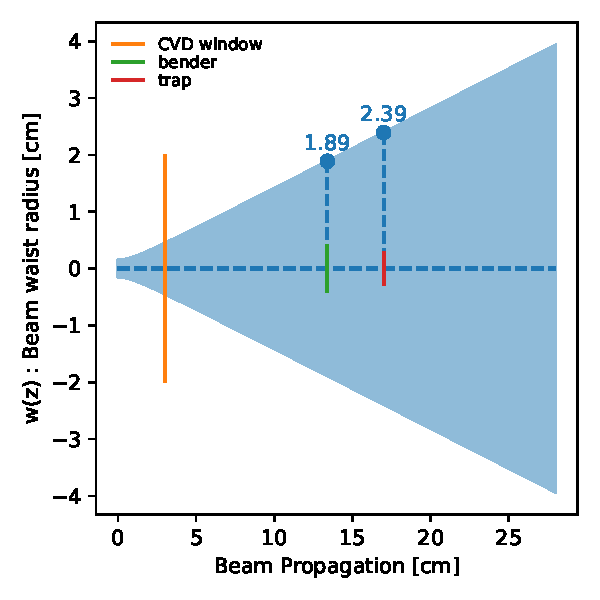
\includegraphics[scale=0.7]{figures/measurements/power-curve-453GHz/beam_propagation.pdf}
    \caption{Gaussian beam (for a frequency of $\nu=453$ GHz) propagation from a beam waist radius of 0.15 cm produced from diagonal feed horn antenna. The solid lines - orange and green indicate the position of the FELion instrument entrance window (CVD diamond window, 3 cm from antenna, 2 cm aperture radius) and bender (10.4 cm from window, 0.43 cm aperture radius), 22-pole ion-trap (14 cm from window, 0.3 cm aperture radius), respectively.}
    \label{fig:power-curve:beam-propagation}
\end{figure}